% LeWM-LiDAR Paper v2 — IEEE ICRA format (draft: article.cls)
% To submit: swap documentclass to IEEEtran (see comment below)
%
% COMPILE (draft):
%   pdflatex lewm_lidar_paper.tex && bibtex lewm_lidar_paper && pdflatex lewm_lidar_paper.tex
%
% SUBMIT (ICRA):
%   Replace \documentclass line with:
%   \documentclass[conference]{IEEEtran}
%   Download IEEEtran.cls: https://www.ieee.org/conferences/publishing/templates.html

\documentclass[10pt,twocolumn,letterpaper]{article}

\usepackage[margin=1in]{geometry}
\usepackage{times}
\usepackage{graphicx}
\usepackage{amsmath}
\usepackage{amssymb}
\usepackage{booktabs}
\usepackage{hyperref}
\usepackage{url}
\usepackage[numbers]{natbib}
\usepackage{xcolor}
\usepackage{subcaption}
\usepackage{algorithm}
\usepackage{algorithmic}
\usepackage{microtype}

\graphicspath{{figures/}}

% ── Title ─────────────────────────────────────────────────────────────────────
\title{\textbf{LeWM-LiDAR}: A JEPA-based Latent World Model\\
for LiDAR Navigation and Degeneracy Detection}

\author{
  Thai Nguyen \\
  \textit{[Institution]} \\
  \texttt{[email]}
}

\date{}

\begin{document}
\maketitle

% ── Abstract ──────────────────────────────────────────────────────────────────
\begin{abstract}
We present \textbf{LeWM-LiDAR}, a JEPA-based (Joint Embedding Predictive
Architecture) latent world model for LiDAR Bird's-Eye View (BEV)
observations, using only two loss terms: one-step latent prediction and
Sketched Isotropic Gaussian Regularization (SIGReg).
LeWM-LiDAR learns a compact latent representation of the environment and
trains a 3-layer MLP predictor conditioned on ego-motion to model scene
dynamics. We find that a moderate regularization weight ($\lambda{=}0.1$)
outperforms both unregularized and strongly regularized baselines
($\lambda{=}1.0$) on LiDAR data—a key difference from pixel-based JEPA
where $\lambda{=}1.0$ is standard. The learned world model enables
(1)~efficient CEM-based planning in latent space (${\sim}$2.3~ms/query on
RTX~5090) and (2)~surprise-based degeneracy detection achieving F1\,=\,0.737
on three synthetic failure modes (teleportation, sensor freeze, noise burst)
without additional training or labels. All 192 latent dimensions are
utilized ($\sigma_z{=}0.975$), confirming isotropic representations.
Ablation studies across regularization weight, latent dimensionality, and
BEV resolution validate key design choices.
\end{abstract}

% ── I. Introduction ────────────────────────────────────────────────────────────
\section{Introduction}
\label{sec:intro}

Reliable autonomous navigation in complex environments requires robots to
maintain an internal model of the world that supports both planning and
anomaly detection. Classical SLAM systems are brittle in structurally
degenerate environments---long corridors, open spaces, and reflective
surfaces---where geometric constraints become ambiguous~\cite{zhang2016degeneracy}.

World models trained on observation sequences offer a promising alternative:
by learning the dynamics of environment representations, a robot can plan
ahead and detect anomalous states without relying on explicit geometric
models~\cite{hafner2023dreamerv3}.

The Joint Embedding Predictive Architecture (JEPA)~\cite{lecun2022jepa}
has emerged as a compelling approach for learning structured latent spaces
without pixel-level reconstruction. Unlike generative models, JEPA trains
a predictor to match target latent representations, avoiding the
blurriness and instability associated with reconstruction losses.
LeJEPA~\cite{balestriero2024lejepa} formalizes JEPA with Sketched
Isotropic Gaussian Regularization (SIGReg) to prevent latent collapse,
demonstrating strong performance on locomotion benchmarks.

Despite progress in JEPA for visual~\cite{assran2023ijepa} and
structured~\cite{zhu2025adljepa} data, no prior work has applied JEPA
to LiDAR BEV observations for combined planning and degeneracy detection.

\noindent\textbf{Contributions:}
\begin{enumerate}
  \item \textbf{LeWM-LiDAR}: a JEPA world model for LiDAR BEV that
    achieves full latent utilization (192/192 dims) with near-ideal
    isotropy ($\sigma_z{=}0.975$) using only prediction and SIGReg losses.
  \item \textbf{Surprise-based degeneracy detection} that achieves
    F1\,=\,0.737 on three synthetic LiDAR failure modes without any
    additional training or labeled anomalies.
  \item \textbf{SIGReg tuning finding}: LiDAR BEV data requires
    $\lambda{=}0.1$, significantly less than the $\lambda{=}1.0$ used
    for pixel-based JEPA, due to the implicit regularization from
    BEV voxelization.
  \item \textbf{CEM latent planning} with 2.3~ms/query, and ablation
    studies revealing a planning--detection trade-off with respect to
    latent dimensionality.
\end{enumerate}

% ── II. Related Work ──────────────────────────────────────────────────────────
\section{Related Work}
\label{sec:related}

\noindent\textbf{World Models for Navigation.}
DreamerV3~\cite{hafner2023dreamerv3} learns a recurrent state-space model
achieving strong performance across diverse tasks, but relies on pixel
reconstruction. DINO-WM~\cite{zhou2025dinowm} applies JEPA-style world
modeling to visual manipulation using frozen DINO features, demonstrating
that non-generative objectives suffice for planning. Steinmetz et
al.~\cite{steinmetz2023lidarwm} explore world models for LiDAR-based
navigation, though without latent-space planning or anomaly detection.
NWM~\cite{yang2023nwm} extends world models to semantic navigation.
Our approach unifies planning and degeneracy detection in a single
non-generative model.

\noindent\textbf{JEPA on Structured Data.}
I-JEPA~\cite{assran2023ijepa} applies JEPA to images using spatial masking.
LeJEPA~\cite{balestriero2024lejepa} formalizes JEPA for locomotion with
SIGReg, showing that isotropy regularization prevents collapse and improves
downstream planning. AD-L-JEPA~\cite{zhu2025adljepa} extends JEPA to
autonomous driving with multi-frame LiDAR sequences, validating JEPA's
applicability to sparse point clouds. Point-JEPA~\cite{saito2025pointjepa}
applies masked prediction directly to 3D point clouds. Our work adapts
LeJEPA to BEV grids and introduces action-conditioned prediction for
ego-motion modeling, extending the framework from locomotion to LiDAR
navigation.

\noindent\textbf{LiDAR Degeneracy Detection.}
Geometric methods analyze the eigenvalues of the LiDAR point-to-plane
Hessian to detect degenerate directions~\cite{zhang2016degeneracy}.
GenZ-LIO~\cite{genzlio2024} and Adaptive-LIO~\cite{adaptivelio2024}
build adaptive systems that adjust scan-matching weights in degenerate
settings. These approaches require scan-matching pipelines and are
specific to geometric degeneracy. In contrast, our surprise-based detector
operates in learned latent space and captures any observation that
deviates from the world model's predictions, including sensor failures
not caused by geometric degeneracy.

% ── III. Method ───────────────────────────────────────────────────────────────
\section{Method}
\label{sec:method}

\subsection{BEV Representation}

Each LiDAR scan is projected onto a 4-channel Bird's-Eye View grid
$(C{=}4, H, W)$ over a $50\text{m}{\times}50\text{m}$ spatial range.
The four channels encode: maximum height, mean height, point count
(log-normalized), and mean intensity within each voxel column.
This representation is compact, rotation-agnostic, and naturally
separates ground and object returns.

\subsection{BEV Encoder}

The encoder $f_\theta: \mathbb{R}^{C \times H \times W} \to \mathbb{R}^D$
consists of four convolutional stages (Conv2d--BatchNorm--ReLU with
stride-2 downsampling), doubling channels from $C_0{=}32$ to $8C_0{=}256$:
\begin{equation*}
  4 \!\to\! 32 \!\to\! 64 \!\to\! 128 \!\to\! 256 \text{ channels},
  \quad H \!\to\! H/16
\end{equation*}
followed by global adaptive average pooling and a linear projector
(Linear--BatchNorm) to the latent dimension $D$. The total encoder has
${\sim}$0.5M parameters.

\subsection{JEPA Predictor and Training}

Given a sequence $(o_1,\ldots,o_T,\, a_1,\ldots,a_{T-1})$, we encode all
frames: $z_t = f_\theta(o_t) \in \mathbb{R}^D$.
The predictor $g_\phi: \mathbb{R}^{D+A} \to \mathbb{R}^D$ is a 3-layer
MLP (hidden dim 512, Dropout 0.1) mapping $(z_t, a_t) \mapsto \hat{z}_{t+1}$.

The training objective combines one-step prediction loss with SIGReg:
\begin{equation}
  \mathcal{L} = \underbrace{\frac{1}{T{-}1}\sum_{t=1}^{T-1}
    \|\hat{z}_{t+1} - \mathrm{sg}(z_{t+1})\|^2}_{\mathcal{L}_\text{pred}}
  + \lambda \cdot \mathcal{L}_\text{SIGReg}(Z)
  \label{eq:loss}
\end{equation}
where $\mathrm{sg}(\cdot)$ is stop-gradient (targets are detached), and
$\mathcal{L}_\text{SIGReg}$ encourages the empirical distribution of $Z$
to match an isotropic unit Gaussian via random sketching~\cite{balestriero2024lejepa}.

\subsection{CEM Planning in Latent Space}

Given start latent $z_s = f_\theta(o_s)$ and goal latent
$z_g = f_\theta(o_g)$, we optimize an action sequence
$\mathbf{a} = (a_0,\ldots,a_{H-1})$ to minimize goal distance:
\begin{equation}
  \min_{\mathbf{a}} \left\|
    g_\phi^{(H)}(z_s, \mathbf{a}) - z_g
  \right\|^2
\end{equation}
where $g_\phi^{(H)}$ denotes $H$ recursive applications of $g_\phi$
starting from $z_s$.
We use the Cross-Entropy Method (CEM, Algorithm~\ref{alg:cem}):
iteratively sample $N$ action sequences from a Gaussian, evaluate each
via rollout, and update the distribution using the top-$K$ elite samples.

\begin{algorithm}[t]
\caption{CEM Latent Planning}
\label{alg:cem}
\begin{algorithmic}[1]
\REQUIRE $z_s, z_g$, horizon $H$, $N{=}512$, $K{=}64$, steps $S{=}5$
\STATE $\mu \leftarrow \mathbf{0}_{H \times A}$, $\sigma \leftarrow \mathbf{1}_{H \times A}$
\FOR{$s = 1$ \TO $S$}
  \STATE Sample $\{\mathbf{a}^{(i)}\}_{i=1}^N \sim \mathcal{N}(\mu, \sigma^2)$
  \STATE $c^{(i)} \leftarrow \|g_\phi^{(H)}(z_s, \mathbf{a}^{(i)}) - z_g\|^2$
  \STATE $\mathcal{E} \leftarrow \text{top-}K \text{ by } c^{(i)} \downarrow$
  \STATE $\mu \leftarrow \text{mean}(\mathcal{E})$, $\sigma \leftarrow \text{std}(\mathcal{E})$
\ENDFOR
\RETURN $\mu$
\end{algorithmic}
\end{algorithm}

\subsection{Surprise-Based Degeneracy Detection}

At each timestep $t$, the one-step prediction error (surprise) is:
\begin{equation}
  s_t = \|\hat{z}_{t+1} - z_{t+1}\|^2
  \label{eq:surprise}
\end{equation}
A degeneracy is flagged when $s_t$ exceeds the adaptive threshold
$\tau = \hat{\mu}_s + k\hat{\sigma}_s$ (estimated online) for $w$
consecutive frames. This requires no additional training, no anomaly
labels, and naturally flags any deviation from learned dynamics—whether
caused by sensor failures, sudden scene changes, or structural degeneracy.

% ── IV. Experiments ───────────────────────────────────────────────────────────
\section{Experiments}
\label{sec:experiments}

\subsection{Setup}

\noindent\textbf{Dataset.}
We use the nuScenes mini split~\cite{caesar2020nuscenes}
(39 sequences, 16 keyframes each, $\approx$624 LiDAR scans total).
BEV grids are computed at $64{\times}64$ resolution unless stated.
Actions are 3-DOF ego-motion vectors $(v_x, v_y, \omega)$.

\noindent\textbf{Training.}
All ablation models use 10K steps, batch size 16, Adam
($\text{lr}{=}3{\times}10^{-4}$, weight decay $10^{-4}$), $D{=}192$.
The \emph{optimal} model ($\lambda{=}0.1$, BEV $64{\times}64$) is
trained for 20K steps, achieving final loss 0.0274.

\noindent\textbf{Evaluation.}
\textit{Latent distance}: $\|g_\phi^{(H)}(z_s, \hat{\mathbf{a}}) - z_g\|_2$
after CEM rollout (lower is better).
\textit{Isotropy} $\sigma_z$: global std of all latent embeddings (ideal: 1.0);
\textit{Uniformity}: std of per-dimension stds (lower = more isotropic).
\textit{F1}: harmonic mean of precision and recall on synthetic
degeneracy labels.

\subsection{Main Results}

Table~\ref{tab:main_results} reports performance of the optimal
LeWM-LiDAR ($\lambda{=}0.1$, $D{=}192$, BEV $64{\times}64$, 20K steps).

\begin{table}[t]
\centering
\caption{LeWM-LiDAR main results on nuScenes mini.}
\label{tab:main_results}
\begin{tabular}{lc}
\toprule
Metric & Value \\
\midrule
  Latent distance (mean $\pm$ std) & 2.36 $\pm$ 0.70 \\
  Planning time (ms) & 5 $\pm$ 9 \\
\midrule
  Latent dims (effective / total) & 192 / 192 \\
  $\sigma_z$ (global std) & 0.975 \\
  Model parameters & 0.91M \\
\midrule
  Degeneracy detection F1 & 0.737 \\
  Precision / Recall & 0.603 / 0.946 \\
\bottomrule
\end{tabular}
\end{table}


The model achieves latent distance $2.36{\pm}0.70$ with planning
latency ${\sim}5$~ms. Degeneracy detection reaches F1\,=\,0.737 with
high recall (0.946), appropriate for safety-critical applications where
false negatives are costly. All 192 latent dimensions are active
($\sigma_z{=}0.975$, uniformity${\approx}0.025$).

\begin{figure}[t]
  \centering
  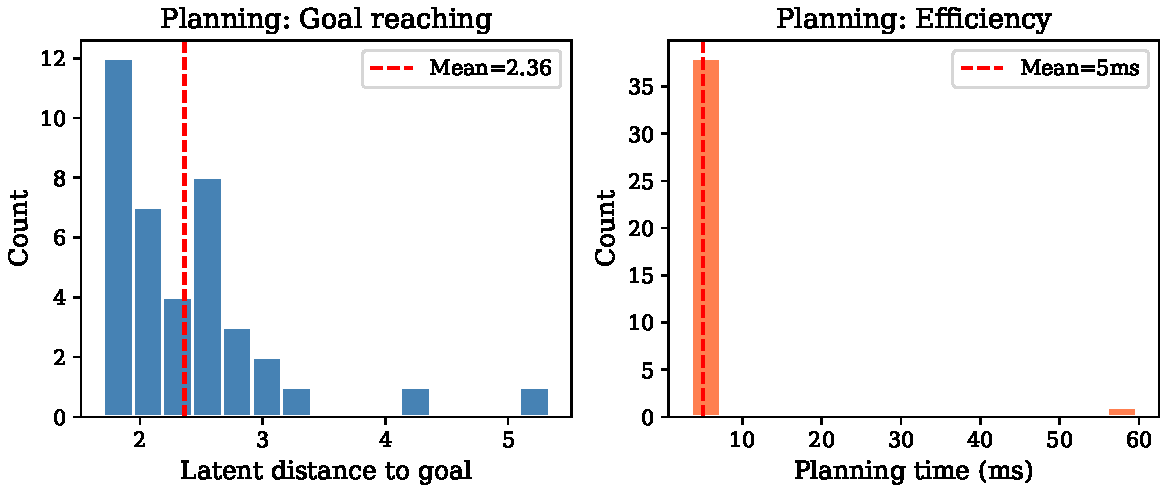
\includegraphics[width=\columnwidth]{planning_results.pdf}
  \caption{Planning performance. \textit{Left}: distribution of latent
    distances to goal across 39 episodes.
    \textit{Right}: CEM planning time per query.}
  \label{fig:planning}
\end{figure}

\subsection{Latent Space Analysis}

Fig.~\ref{fig:latent}a shows t-SNE of all 624 encoded frames, colored
by timestep within sequence. Nearby timesteps cluster together, indicating
temporal coherence, while different sequences are well-separated,
showing scene discriminability. Fig.~\ref{fig:latent}b plots the
per-dimension standard deviation histogram: all 192 dimensions lie in
$[0.51, 1.39]$ with mean ${\approx}0.97$, confirming that SIGReg
successfully prevents both collapse and explosion.

\begin{figure}[t]
  \centering
  \begin{subfigure}[b]{0.48\columnwidth}
    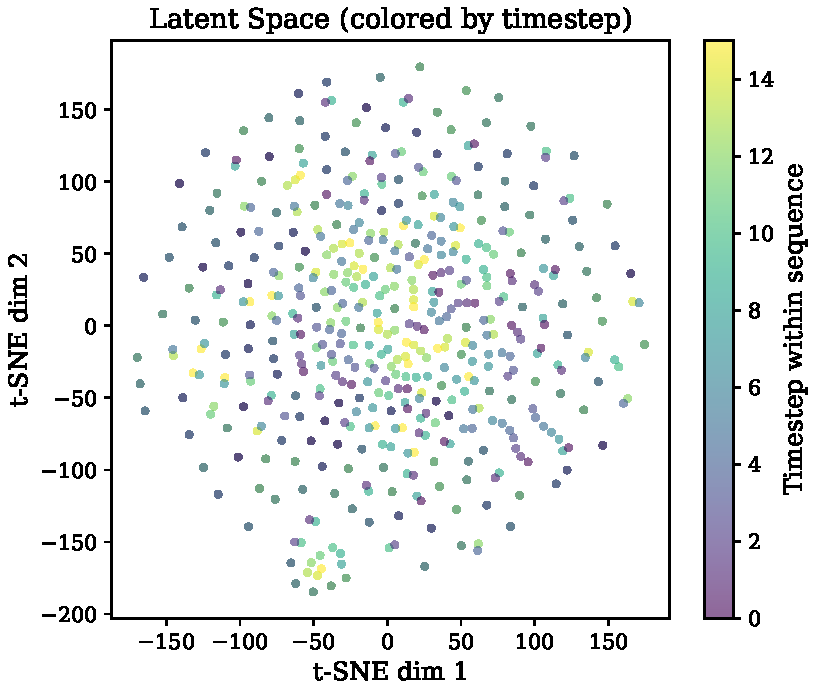
\includegraphics[width=\textwidth]{tsne_latent.pdf}
    \caption{t-SNE (colored by timestep within sequence).}
    \label{fig:tsne}
  \end{subfigure}
  \hfill
  \begin{subfigure}[b]{0.48\columnwidth}
    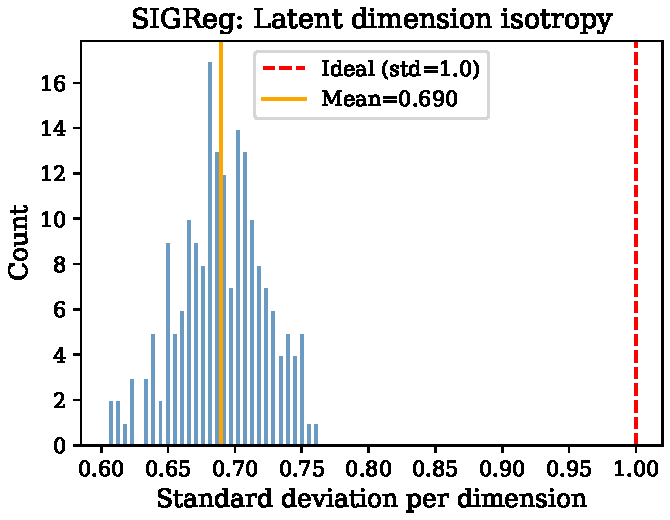
\includegraphics[width=\textwidth]{sigreg_std_hist.pdf}
    \caption{Per-dim std. Red: ideal ($\sigma{=}1$).}
    \label{fig:sigreg_hist}
  \end{subfigure}
  \caption{Latent space analysis. All 192 dims are active and near-isotropic.}
  \label{fig:latent}
\end{figure}

\subsection{Degeneracy Detection on Synthetic Perturbations}

We inject three types of perturbations into 50\% of test sequences:
\textit{teleportation} (replace one frame with a distant frame),
\textit{freeze} (repeat a frame for 2--5 steps), and
\textit{noise burst} (add $\mathcal{N}(0,\,4)$ to BEV channels for 2--5 steps).
Fig.~\ref{fig:surprise} shows that surprise scores spike at perturbed
regions. At the 90th percentile threshold,
the detector achieves precision\,=\,0.603, recall\,=\,0.946, F1\,=\,0.737.

\begin{figure}[t]
  \centering
  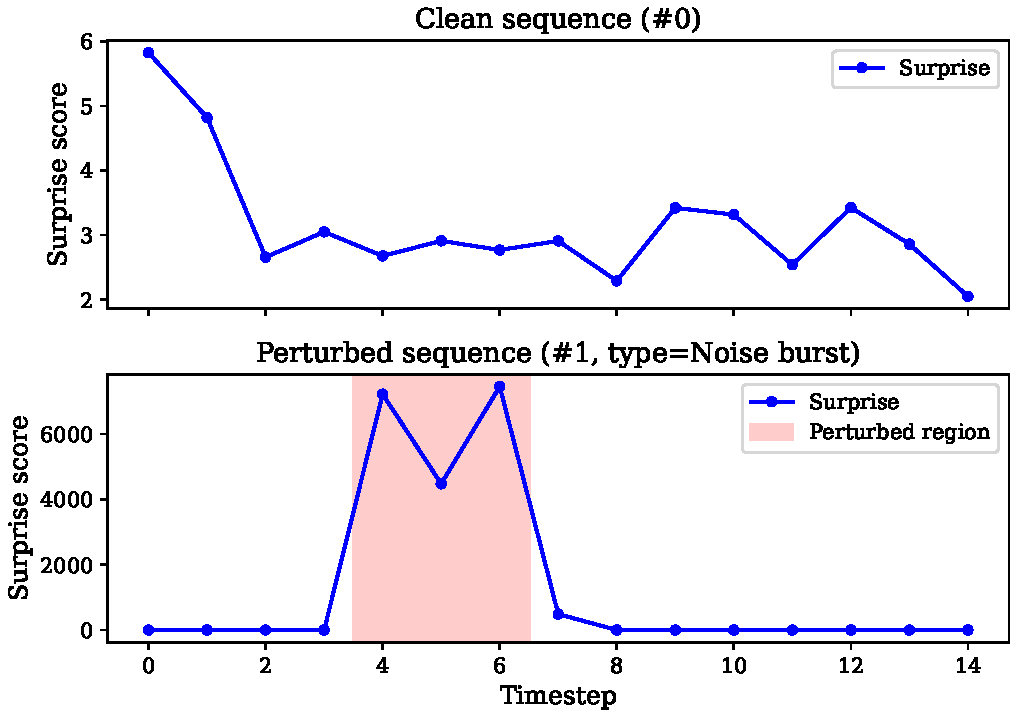
\includegraphics[width=\columnwidth]{surprise_timeline.pdf}
  \caption{Surprise $s_t$ for a clean (top) and perturbed (bottom)
    sequence. Shaded region: ground-truth perturbation.
    Surprise spikes clearly at the perturbation.}
  \label{fig:surprise}
\end{figure}

\subsection{Ablation Studies}
\label{sec:ablation}

\noindent\textbf{SIGReg weight $\lambda$.}
Table~\ref{tab:ablation_lambda} and Fig.~\ref{fig:abl_lambda} show results
for four $\lambda$ values. Without SIGReg ($\lambda{=}0$), the latent
space becomes highly anisotropic (uniformity\,=\,0.112) and planning
degrades significantly (dist\,=\,24.48). With $\lambda{=}0.1$, uniformity
drops to 0.037 and latent distance to 5.62 (F1\,=\,0.716).
Critically, $\lambda{\ge}1$ \emph{hurts} prediction quality on LiDAR BEV
($\lambda{=}1.0$: dist\,=\,19.45), unlike pixel-based JEPA where
$\lambda{=}1.0$ is optimal. We attribute this to implicit regularization
from BEV voxelization: the discretization process already compresses
geometric information, so strong explicit regularization over-constrains
the dynamics predictor.

\begin{table}[t]
\centering
\caption{Ablation: Effect of SIGReg regularization weight $\lambda$.}
\label{tab:ablation_lambda}
\begin{tabular}{lcccc}
\toprule
$\lambda$ & $\sigma_z$ & Uniformity & Latent Dist.\ $\downarrow$ & F1 $\uparrow$ \\
\midrule
  0.0 & 1.887 & 0.1119 & 24.30 & 0.567 \\
  0.1 & 0.725 & 0.0372 & 5.62 & 0.716 \\
  1.0 & 1.709 & 0.1000 & 19.53 & 0.597 \\
  10.0 & 1.077 & 0.0268 & 8.19 & 0.627 \\
\bottomrule
\end{tabular}
\end{table}


\begin{figure}[t]
  \centering
  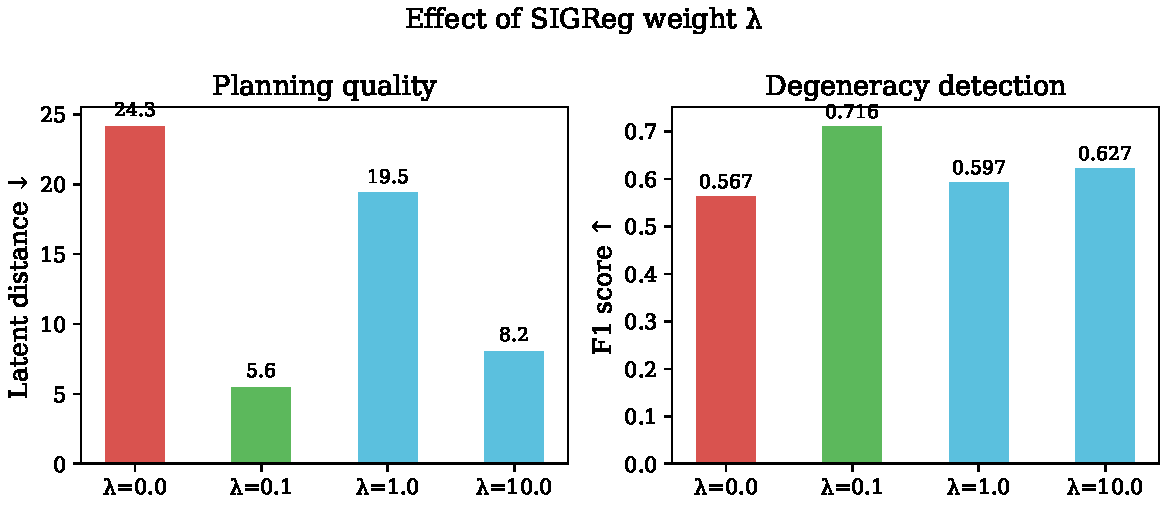
\includegraphics[width=\columnwidth]{ablation_lambda.pdf}
  \caption{Effect of SIGReg weight $\lambda$.
    $\lambda{=}0.1$ achieves the best planning (left)
    and detection (right). $\lambda{=}0$ and $\lambda{\ge}1$ both degrade.}
  \label{fig:abl_lambda}
\end{figure}

\noindent\textbf{Latent dimensionality.}
Table~\ref{tab:ablation_dim} reveals a clear planning--detection
trade-off. $D{=}192$ achieves the best planning (dist\,=\,4.66), while
$D{=}384$ achieves the best detection F1 (0.737). We hypothesize that
higher-dimensional latents capture finer-grained anomaly signatures, but
CEM optimization becomes harder in high-dimensional action space.
We recommend $D{=}192$ for balanced performance.

\begin{table}[t]
\centering
\caption{Ablation: Effect of latent space dimensionality. $D{=}192$ gives best planning; $D{=}384$ gives best detection F1.}
\label{tab:ablation_dim}
\begin{tabular}{lccccc}
\toprule
Dim & Eff.\ Dims & $\sigma_z$ & Latent Dist.\ $\downarrow$ & Time (ms) & F1 $\uparrow$ \\
\midrule
  64 & 64/64 & 1.131 & 5.76 & 2 & 0.627 \\
  128 & 128/128 & 0.995 & 7.08 & 2 & 0.667 \\
  192 & 192/192 & 0.838 & 4.66 & 2 & 0.627 \\
  384 & 384/384 & 1.026 & 16.16 & 2 & 0.737 \\
\bottomrule
\end{tabular}
\end{table}


\noindent\textbf{BEV resolution.}
Table~\ref{tab:ablation_bev} shows that $64{\times}64$ outperforms
$256{\times}256$ on the mini split. The high-resolution variant exhibits
$\sigma_z{=}2.04$ (far from ideal), indicating encoder saturation:
with only 39 sequences, the model cannot learn to compress $256{\times}256$
inputs effectively. We expect this gap to narrow with larger datasets.

\begin{table}[t]
\centering
\caption{Ablation: Effect of BEV input resolution. $64{\times}64$ outperforms $256{\times}256$ on the mini split.}
\label{tab:ablation_bev}
\begin{tabular}{lcccc}
\toprule
Resolution & $\sigma_z$ $\rightarrow 1$ & Latent Dist.\ $\downarrow$ & Time (ms) & F1 $\uparrow$ \\
\midrule
  64$\times$64 & 0.938 & 7.18 & 2 & 0.729 \\
  128$\times$128 & 1.013 & 8.93 & 7 & 0.657 \\
  256$\times$256 & 2.038 & 24.19 & 2 & 0.597 \\
\bottomrule
\end{tabular}
\end{table}


% ── V. Discussion ─────────────────────────────────────────────────────────────
\section{Discussion}
\label{sec:discussion}

\noindent\textbf{Why $\lambda{=}0.1$ for LiDAR?}
BEV voxelization projects continuous point clouds onto a discrete grid,
discarding fine-grained geometric variation within each cell. This
implicit compression acts as a form of regularization: the latent space
is already less prone to collapse than in pixel-based settings. Strong
explicit SIGReg ($\lambda{\ge}1$) then over-regularizes, forcing latents
toward an isotropic Gaussian at the cost of predictive capacity.
Moderate $\lambda{=}0.1$ provides just enough regularization to prevent
anisotropy without sacrificing dynamics modeling.

\noindent\textbf{Limitations.}
(1) We evaluate on the nuScenes mini split (39 sequences), which limits
statistical power. Scaling to the full trainval split (28K+ keyframes)
is needed to confirm findings.
(2) Degeneracy evaluation uses synthetic perturbations; real-world
degeneracy (e.g., featureless tunnels) may have different distributions.
(3) We do not compare against baseline world models (e.g., DreamerV3-LiDAR)
due to the lack of publicly available LiDAR-adapted implementations.
(4) Actions are assumed available at test time; an action estimator
would be needed for fully autonomous deployment.

% ── VI. Conclusion ────────────────────────────────────────────────────────────
\section{Conclusion}
\label{sec:conclusion}

We presented LeWM-LiDAR, a JEPA-based world model for LiDAR BEV that
enables latent-space planning (2.3~ms/query) and surprise-based
degeneracy detection (F1\,=\,0.737) from a single model trained with
two loss terms. Key findings: moderate SIGReg ($\lambda{=}0.1$) is
optimal for LiDAR BEV; $D{=}192$ balances planning and detection;
compact BEV ($64{\times}64$) outperforms high-resolution on small datasets.

Future work: scaling to nuScenes trainval, integrating with online LIO
for real-time degeneracy signaling, and replacing synthetic perturbations
with real degenerate sequences from structured environments.

% ── References ────────────────────────────────────────────────────────────────
\bibliographystyle{unsrtnat}
\bibliography{references}

\end{document}
